\documentclass[Bachelorarbeit.tex]{subfiles}
\begin{document}
\chapter{Evaluation}
\label{chap:evalutation}
Nach der Implementierung des Prototypen, gilt es festzustellen ob und welchen Mehrwert das System für Anwender\_innen darstellt. 
Für diesen Zweck, sowie um etwaige Schwachstellen zu identifizieren, soll der Prototyp im Rahmen einer Usability-Analyse auf seine Effektivität, Effizienz und Zufriedenstellung \cite[vgl.][Abs.: 3]{Iso9241_11} untersucht werden (siehe Abschnitt: \nameref{Methodik}).
Zusätzlich zur Usability-Analyse soll auch die Art und Weise untersucht werden, wie die verschiedenen Ansichten (Karte und Liste) während des Tests verwendet werden.\\
\\
Der Ablauf der Usability-Analyse sieht wie folgt aus:
Im ersten Schritt werden die zu untersuchenden Kriterien (siehe Absatz: \nameref{Usability}) erläutert.
Darauf folgt die Festlegung und Beschreibung der Verfahren welche zum Messen ebendieser Kriterien angewandt werden.
Basierend auf den definierten Verfahren, wird die Erstellung und Begründung für die Auswahl des Testmaterials dargelegt, welche auch im Anhang zu finden ist (siehe Anhang: \ref{anhangTestmaterial} - \nameref{anhangTestmaterial}).
Im Abschnitt \nameref{Stichproben} wird der Rahmen für die Tests, sowie die Auswahl der Proband\_innen festgelegt.
Die anschließende Dokumentation, sowie die Ergebnisse der Durchführung werden im Abschnitt \nameref{Ergebnisse} behandelt.
Abschließend findet eine \nameref{InterpretationDiskussion} auf der Basis der Ergebnisse statt, die zum einen die Evaluation der \nameref{Hypothese} und zum anderen den Mehrwert der wählbaren Ansichten  klärt.

\section{Methodik}
\label{Methodik}

Da die Interviews im Vorfeld ergeben haben, dass jede befragte Person einen unterschiedlichen Ablauf sowie unterschiedliche Werkzeuge bei der Planung der Außendienstrouten einsetzt, hilft ein vergleichender Test zwischen dem Status Quo und dem Prototypen an dieser Stelle nicht weiter.
Aus diesem Grund liegt es nahe einen klaren Schnitt zu den diversen alten Systemen zu ziehen und eine Formative Usability Evaluation\footnote{Bei der Formativen Evaluation wird anhand definierter Kriterien untersucht, ob der Entwurf weiter optimiert werden kann. (vgl. \cite{Burmester}, S. 343)} nach den Kriterien der ISO 9241 durchzuführen.
Dafür soll der Prototyp auf die nachfolgende Hypothese hin mit benutzerorientierten Methoden\footnote{Dabei liegt der Fokus bei den Tests auf definierten Anwender\_innen-Gruppen. (vgl. \cite{Burmester}, S. 343)} untersucht werden.


\subsection{Hypothese}
\label{Hypothese}

Der Prototyp unterstützt die potentiellen Pery-Anwender\_innen messbar in den Bereichen Effektivität, Effizienz und Zufriedenstellung bei der Planung von Außendiensteinsätzen (Die Begriffe Effektivität, Effizienz und Zufriedenstellung beziehen sich auf die Definition nach der Norm EN ISO 9241-11, \cite[vgl.][Abs.: 3]{Iso9241_11}).


\subsection{Exkurs Usability}  
\label{Usability}
Durch den sinnvollen Einsatz von Usability-Maßnahmen in der Entwicklung lässt sich die Qualität eines Produktes spürbar erhöhen.
Neben der Steigerung der Produktivität und der Zufriedenheit der Anwender\_innen werden laut Burmester auch die Einschulungszeiten am Produkt deutlich verringert (\cite[vgl.][352f]{Burmester}).\\
\\
Im deutschsprachigen Raum werden die zwei Begriffe Gebrauchstauglichkeit und Softwareergonomie in Kontext mit Usability gesetzt.
Dabei gilt es allerdings zu beachten, dass der Begriff Softwareergonomie über den Umfang der Gebrauchstauglichkeit hinausreicht und beispielsweise auch Korrektheitsergonomie und Funktionsergonomie umfasst
(\cite[vgl.][420]{Niegemann2008})\\
\\
Innerhalb dieser Arbeit wird der Begriff Usability im Kontext der Gebrauchstauglichkeit verwendet, die wie folgt in der ISO 9241 definiert wurde (\cite[siehe:][Abs.: 3.1 Gebrauchstauglichkeit]{Iso9241_11}):

\begin{quote}
	"\textit{Das Ausmaß, in dem ein Produkt durch bestimmte Benutzer in einem bestimmten Nutzungskontext genutzt werden kann, um bestimmte Ziele effektiv, effizient und zufriedenstellend zu erreichen.}" 
\end{quote}

Somit ergibt laut dieser Definition die Usability-Evaluation (Analyse in Bezug auf Gebrauchstauglichkeit), inwiefern der Prototyp (Produkt) die Anwender\_innen bei der Planung von Außendienstrouten (Nutzungskontext) unterstützt.
\pagebreak
\paragraph{Effektivität}
Die Effektivität beschreibt, ob und wie es möglich ist die gestellte Aufgabe innerhalb des Nutzungskontext zu lösen.
Für diesen Zweck muss betrachtet werden, inwiefern die Funktionalität des Prototyps die Anwender\_innen bei dem erreichen des Ziels, innerhalb eines definierte Szenarios unterstützt (vgl. \cite{Iso9241_11}, S. 4 sowie \cite{Burmester}, S. 325). \\
\\
Ein Negativbeispiel anhand des Prototyps könnte wie folgt aussehen:
Die Aufgabenstellung verlangt, dass alle Kunden ausgewählt werden sollen, die innerhalb des letzten 24 Stunden Bestellungen aufgegeben haben. 
Wenn der Prototyp allerdings nur die Möglichkeit anbietet Kunden anzuzeigen, die innerhalb der letzten Woche bestellt haben, kann das Ziel nicht erfüllt werden und ist somit nicht effektiv.

\paragraph{Effizienz}
Die Effizienz beschreibt wie viel Aufwand für die Lösung der Aufgabe innerhalb des Nutzungskontext nötig ist. 
Dabei trägt neben der Funktionalität das \ac{UI} (beispielsweise die Übersichtlichkeit und Erforschbarkeit) des Prototypen eine tragende Rolle, inwiefern Anwender\_innen zügig und sicher eine Aufgabe bewältigen können (vgl. \cite{Iso9241_11}, S. 4 sowie \cite{Niegemann2008}, S. 421f).\\
\\
Ein Beispiel anhand des Prototypen könnte wie folgt aussehen:
Die Aufgabenstellung gibt an, dass ein Partnerkontakt besucht werden soll. Zusätzlich soll evaluiert werden, welche weiteren Partnerkontakte sich in der Nähe (Umkreis ca. 1 km) befinden, dabei sollen Adressen auch städteübergreifend  berücksichtigt werden (siehe Abb.: \ref{fig:HarteGrenzen} in Kapitel \nameref{chap:entwicklung} für die Visualisierung des Problems).
Durch die Bereitstellung einer Kartenansicht kann in diesem Fall die Effizienz deutlich gesteigert werden. 

\paragraph{Zufriedenstellung}
Zufriedenstellung ist gegeben, wenn Anwender\_innen nicht durch das System behindert werden und eine positive Meinung über das Produkt haben. (vgl. \cite{Burmester}, S. 326)
Dies ist unter anderem zu erreichen, indem die Erwartungshaltung der Anwender\_innen gegenüber dem Produkt (Funktionsumfang und \ac{UI}) erfüllt wird.
Des Weiteren ist es zu vermeiden, Anwender\_innen durch aufwendige Dialoge oder einen unstrukturierten Aufbau des \ac{UI}s in ihrem Arbeitsfluss zu beeinträchtigen.
Dadurch stellt sich laut Niegemann eine subjektiv positive Haltung ein, was wiederum die Grundlage für die Akzeptanz des Produktes darstellt (vgl. \cite{Iso9241_11}, S. 4 sowie \cite{Niegemann2008}, S. 422).\\
\\
Ein mögliches Negativbeispiel kann ein unerwartetes Verhalten der Applikation sein.
In der Kartendarstellung des Prototypen werden verschiedene Adressen auf der Karte dargestellt, dabei handelt es sich zum einen um Kunden- und zum anderen um Lieferantenadressen. 
Wenn sich das Verhalten beim Klick auf einen der Marker für die Anwender\_innen auf unlogische Weise voneinander  unterscheidet\footnote{Beispielsweise wird bei einem Klick auf einen Kunden ein Popup und bei einem Lieferanten eine vollständige Detailansicht (welche die Kartenansicht ersetzt) geöffnet.} ist dies irritierend und hemmt die Anwender\_innen in ihren Arbeitsfluss.
Das wiederum hat zur Folge, dass sich keine Zufriedenstellung einstellt und auch keine Akzeptanz gegenüber dem Produkt etabliert.


\paragraph{Nutzungskontext}

Ein weiterer wichtiger Punkt stellt der Nutzungskontext dar, der den Rahmen definiert in dem die Evaluation durchgeführt wird.
Anhand der ISO 9241 wird der Nutzungskontext wie nachfolgend definiert (siehe \cite{Iso9241_11}, S. 4). 

\begin{quote}
\textit{"Die Benutzer, die Arbeitsaufgaben, Arbeitsmittel (Hardware, Software und Materialien) sowie die physische und soziale Umgebung, in der das Produkt genutzt wird."}
\end{quote} 

Somit wird anhand der Tests nicht eine allgemeine Gebrauchstauglichkeit evaluiert, sondern ausschließlich die Gebrauchstauglichkeit des Produkts für den jeweils definierten Nutzungskontext.

\subsection{Verfahren}
\label{Verfahren}
Um den Prototypen auf die Gebrauchstauglichkeit (siehe Absatz \nameref{Usability}) hin zu untersuchen, muss geklärt werden, wie die Kriterien Effektivität, Effizienz und Zufriedenstellung sinnvoll gemessen werden können. 
Zu diesem Zweck werden an dieser Stelle die Verfahren definiert und erläutert, welche die Grundlage für die Datenerhebung darstellen.

\paragraph{Effektiv}
In erster Linie soll die Effektivität mit Hilfe des \nameref{Eyetracking}-Verfahrens ermittelt werden.
Dabei wird in der Auswertung analysiert, ob die Testpersonen die gestellten Aufgaben mithilfe des Prototypen bewältigen konnten.
Ergänzend zum \nameref{Eyetracking} erfolgt eine subjektive Einschätzung anhand eines geführten \nameref{FragebogenEvaluation}s. 

\paragraph{Effizient}
Auch im Bereich der Effizienz basiert die Analyse verstärkt auf dem \nameref{Eyetracking}-Verfahren, welches durch die Erhebung des \nameref{FragebogenEvaluation}s um die persönliche Meinung, sowie Anmerkungen der Testpersonen erweitert wird.
Mit Hilfe des \nameref{Eyetracking}s soll analysiert werden, ob sich die Bearbeitungsdauer der einzelnen Testfälle linear zu deren Schwierigkeitsgrad verhält. 

\paragraph{Zufriedenstellend}
Im Gegensatz zur Effektivität und der Effizienz verhält sich Messung der Zufriedenstellung subjektiv, da es kein objektives Messkriterium gibt, welches evaluiert werden kann.
Laut Burmester ist dieses Ziel erreicht, wenn die Testpersonen durch den Prototypen nicht behindert werden und sich bei ihnen ein positives Gefühl einstellt (vgl. \cite{Burmester}, S. 326). 
Für die Analyse dieser Dimension werden zum einen Fragen im Rahmen des Fragebogens gestellt und zum anderen Bemerkungen der Testpersonen während des \nameref{Eyetracking}-Tests aufgezeichnet.
Im Anschluss an den Fragebogen soll geklärt werden, ob diese Bemerkungen einer subjektiv positiven oder negativen Einstellung zuzuordnen sind.

\paragraph{Nutzungskontext}
\label{Nutzungskontext}
Die Testperson, welche eine natürliche Person mit Interesse an der Software Pery ist, soll selbständig mit Hilfe des entwickelten Prototypen verschiedener Szenarios der Außendienstplanung durchführen. 
Im Vorfeld dazu findet eine kurze mündlichen Einführung durch eine betreuende Person (Perfany Mitarbeiter\_in und/oder verantwortliche Person im Unternehmen) statt.
Bei Problemen, welche die Effektivität gefährden, kann eine mündliche Nachfrage (telefonischer Support oder direktes Gespräch) mit einer betreuenden Person erfolgen. 
Für die Bearbeitung stehen der Person ein geeigneter Computerarbeitsplatz (PC, Monitor und benötigte Peripheriegeräte), ein funktionstüchtiger und aktueller Webbrowser (Mozilla Firefox oder Google Chrome) sowie eine funktionierende Internetverbindung zur Verfügung.


\subsubsection{Eyetracking}
\label{Eyetracking}

Eyetracking gibt uns die Möglichkeit objektive Daten über das Verhalten der Anwender im Kontext der Interaktion mit dem System zu erhalten.
Während in Tests ohne Eyetracking meist klassische Benutzeraktionen, wie beispielsweise die Interaktion mit Eingabegeräten (z.B. Maus und Tastatur) oder Kameraaufzeichnungen des Bildschirms und der Proband\_innen erfasst werden, können durch Eyetracking zusätzliche Informationen, wie das Verhalten der Testpersonen evaluiert werden.
Diese zusätzlichen Messdaten geben Ausschluss darüber, ob und in welcher Reihenfolge Informationen des \ac{UI}s durch die Proband\_innen wahrgenommen wurden. (vgl. \cite{Niegemann2008}, S. 439ff und \cite{Burmester}, S. 347ff)\\
\\
Das menschliche Auge arbeitet mit zwei Zuständen: Fixation und Sukkaden.
Bei der Fixation blickt das Auge auf einen Punkt und es findet die Informationsverarbeitung statt. 
Während bei der Sukkade der Blick zur nächsten Informationsquelle springt bei der anschließend wieder eine Fixation stattfindet. (vgl. \cite{Burmester}, S. 347f)\\
\\
Durch diesen Effekt kann mit Hilfe des Eyetrackingssystems eine Blickabfolge erstellt und ausgewertet werden (siehe Abb.: \ref{fig:Eyetracking}-1).
Zusätzlich zu der Blickabfolge können auch sogenannte Heatmaps erstellt werden. 
Diese visualisieren wie lange auf bestimmte Bereiche des Monitors geblickt wurde (siehe Abb.: \ref{fig:Eyetracking}-2).
Mithilfe der Auswertung dieser beider Analysen erhalten wir schlussendlich Informationen darüber, welche Inhalte (z.B. Steuer- oder Navigationselemente) wie schnell und sicher gefunden wurden und ob es Ablenkungen gab. (vgl. \cite{Niegemann2008}, S. 439ff und \cite{Burmester}, S. 347ff)

 

\begin{figure}[H]
\centering
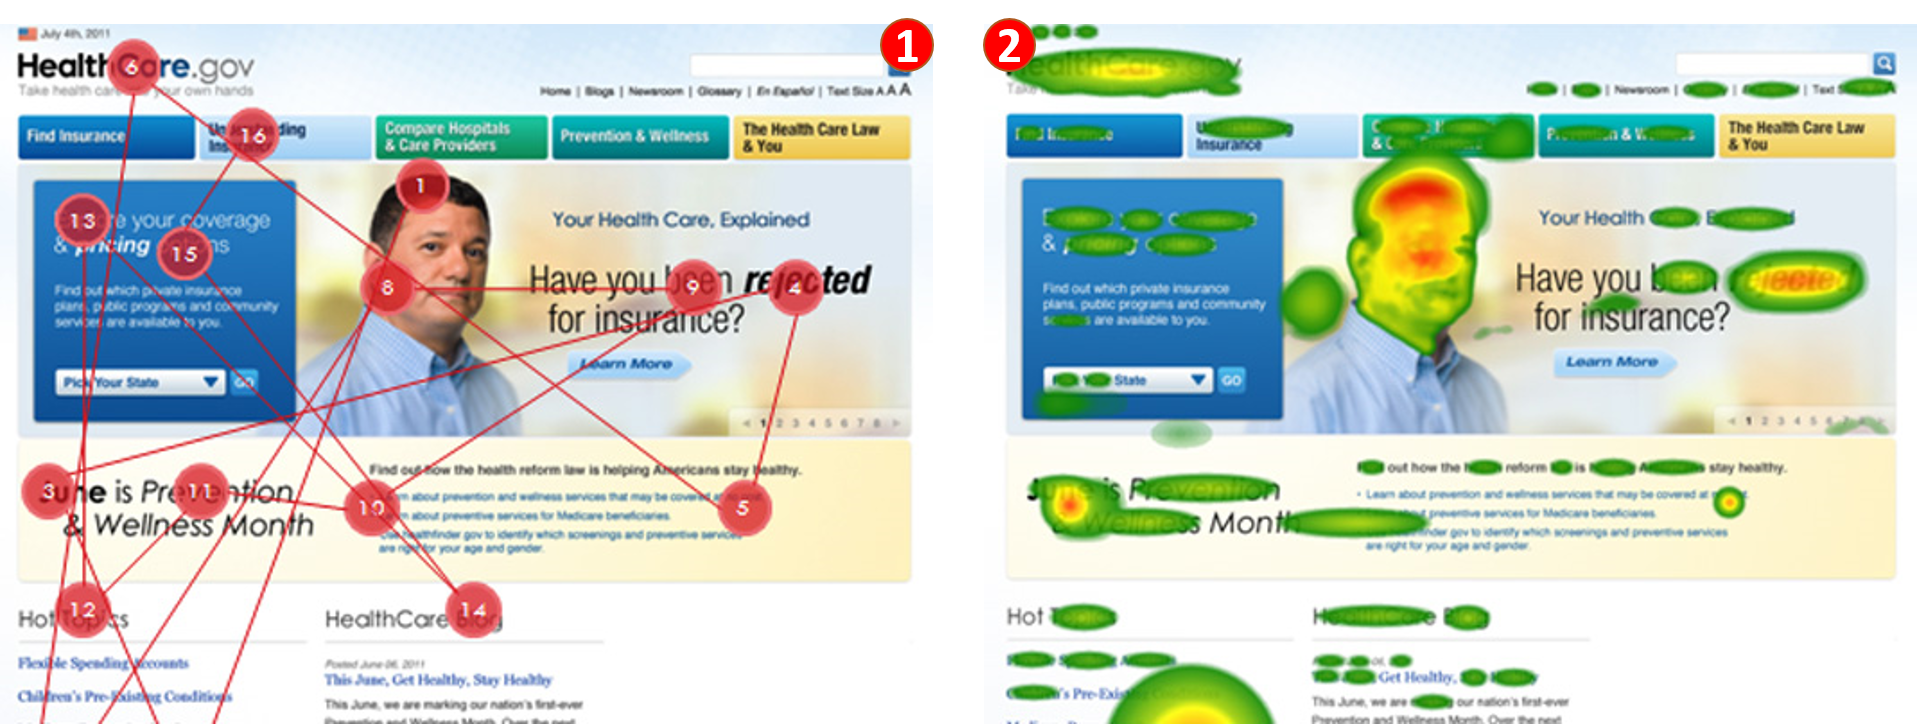
\includegraphics[width=1\linewidth]{img/Evaluation/Eyetracking}
\caption[Auswertungen der Eyetrackinganalyse]{Auswertungen der Eyetrackinganalyse. Linkes Bild (Marker 1): Ansicht einer ausgewerteten Blickabfolge. Rechtes Bild (Marker 2): Ansicht einer ausgewertet Heatmap (Quelle: https://www.usability.gov/how-to-and-tools/methods/eye-tracking.html - Stand Sommer 2016)}
\label{fig:Eyetracking}
\end{figure}


\subsubsection{Fragebogen}
\label{FragebogenEvaluation}


Während beim Eyetracking objektive Messungen  (Dauer des Ablaufs, Blickreihenfolge, etc.) durchgeführt werden, stellt die Methode des Fragebogens eine subjektive Messung dar.
Da der Faktor Zufriedenheit in erste Linie subjektiv ist, wird dieser mit Hilfe des Fragebogens analysiert (vgl. \cite{Ollermann2007}, S. 57).
Zusätzlich besteht aus Sicht der Evaluierung die Notwendigkeit, weitere Informationen, wie beispielsweise Selbsteinschätzungen oder Anmerkungen zum Prototypen, ergänzend zum Eyetracking erheben (vgl. \cite{Laugwitz2006}, S. 127). \\
\\
Einer der Vorteile der Methode des Fragebogens liegt unter anderen in der guten Auswertbarkeit der erhobenen Daten - speziell beim Einsatz von geschlossenen Fragen\footnote{Bei geschlossenen Fragen können die Proband\_innen ausschließlich auf vordefinierte Antworten zurückgreifen (vgl. \cite{Ollermann2007}, S. 61)} (vgl. \cite{Ollermann2007}, S. 61). 
Bei der Erstellung des Fragebogens ist darauf zu achten, dass es sich nicht  um eine willkürliche Ansammlung von Fragen handelt.
Die Verwendung von Fragebögen birgt auch Nachteile, welche unterstreichen, dass es sich um ein subjektives Verfahren handelt, wie Ollemannn in den nachfolgenden vier Punkten skizziert.
\begin{itemize}
	\item Beim Halo-Effekt haben Anwender\_innen die Tendenz konkrete Merkmale aufgrund  eines globalen Pauschalurteils (z.B. Einschätzung der Gebrauchstauglichkeit anhand rein ästhetischer Gesichtspunkte) zu fällen.
	\item Die Abgabe von systematisch zu positiven oder negativen Bewertungen (Milde-Härte-Fehler).
	\item Das Gegenteil davon ist die zentrale Tendenz. Dabei werden Bewertungen vorwiegend im mittleren Bereich der Skala abgeben.
	\item Beim Primacy-Recency-Effekt wird die Bewertung durch die Reihenfolge der einzelnen Fragen beeinträchtigt. 
\end{itemize}
(siehe \cite{Ollermann2007}, S. 60)\\
\\
Damit der Fragebogen als funktionales Werkzeug bei der Evaluierung eingesetzt werden kann, empfiehlt Burmester die Beachtung von Gütekriterien bei der Erstellung.
Dabei handelt es sich um das Gütekriterium der Validität\footnote{Der Fragebogen sollte darauf ausgelegt sein, dass zu messen was er vorgibt. (nach \cite{Burmester}, S. 350)}, das Gütekriterium der Reliabilität\footnote{Ein wiederholtes Durchführen, unter den gleichen Bedingungen, soll zu dem selben Ergebnis führen. (nach \cite{Burmester}, S. 350)} und das Gütekriterium der Objektivität\footnote{Das Ergebnis ist unabhängig von der Person, welche die Untersuchung durchführt. (nach \cite{Burmester}, S. 350)}. \\



\subsection{Aufbau der Evaluation}
Anhand der Evaluation soll zum einen untersucht werden, ob der Prototyp den Anforderungen der Usability-Standards (Gebrauchstauglichkeit)\footnote{Gebrauchstauglichkeit nach ISO 9241 (\cite[siehe:][Abs.: 3.1 Gebrauchstauglichkeit]{Iso9241_11})} entspricht und zum anderen, wie die Testpersonen die einzelnen Darstellungsformen der Daten (Karten- und Listenansicht) einsetzen und verwenden.
Dabei ist die Evaluation in die drei Teilbereiche Einführung, Eyetracking-Test und Fragebogen untergliedert.

\paragraph{Einführung der Testpersonen}
Aufgrund des unterschiedlichen Wissensstände der Testpersonen\footnote{Es wurden unter andern Personen ausgewählt die weder Erfahrung mit Pery haben und/oder in den Entstehungsprozess des Prototyps involviert waren.}, ist es notwendig einen gemeinsamen Nenner zu finden. Das soll mit Hilfe der Einführung realisiert werden soll.\\
\\
Im ersten Teil der Einführung werden Testpersonen, denen Pery fremd ist, die Hintergründe von Perfany und der grobe Funktionsumfang von Pery erläutert.
Der zweite Teil beschäftigt sich damit Testpersonen mit den Szenario vertraut zu machen.
Dabei wird ihnen erklärt, dass Sie im Außendienst tätig sind und anhand der gegeben Aufgabenstellung sowie mit Hilfe des Prototypen eine Menge an Partnerunternehmen für Außendiensteinsätze auswählen sollen.
Im dritten Teil werden im Groben die Funktion und die unterschiedlichen Bereiche des \ac{UI}s vorgestellt. 
Diese Einführung wird ausschließlich mündlich und nicht am Prototypen durchgeführt, um Platz für eigene Erkundungsversuche beim Test einzuräumen.
Abschließend wird die Aufgabenstellung für den Eyetracking-Test erläutert und eventuelle Unklarheiten beseitigt.


\paragraph{Eyetracking-Test}
Um ein möglichst realistisches Ergebnis der Tests für die Evaluation zu erhalten, orientiert sich der Aufbau soweit möglich an den realen Bedingungen, welche im Abschnitt \nameref{Nutzungskontext} beschrieben werden.
Abweichungen bei der Größe- und Auflösung des Monitors oder des Webbrowsers in dem der Prototyp verwendet wird zu unterschiedlichen Darstellungen führen. 
Dies kann wiederum dazu führen das weniger Informationen angezeigt werden wodurch die Effizienz eingeschränkt wird. (vgl. \cite{Ollermann2007}, S. 40)\\
\\
Für den Test wurde folgende Aufbau verwendet:
\begin{enumerate}
	\item Laptop mit installierter Tobii Software Suite\footnote{Wird verwendet um den Eyetracking Test aufzuzeichnen.}
	\item 24 Zoll Monitor mit einer Auflösung von 1920x1080 Pixel
	\item Mozilla Firefox
	\item Webcam mit Mikrophon für die Aufzeichnung der Testperson während des Testes
\end{enumerate}

Der Test selbst ist in drei Stufen unterteilt, wobei bei jeder Stufe die Komplexität der Aufgaben erhöht wird. 
In jeder der drei Problemstellungen ist die Testperson angehalten einen Außendiensteinsatz zu planen. 
Die jeweilige Schwierigkeit wird dabei durch die zusätzlichen Bedingungen definiert.
Anhand dieser Vorgehensweise soll anschließend ermittelt werden, wie sich die Bearbeitungsdauer, unter der Berücksichtigung des Erfahrungsgrades der Testperson, verhält. \\
\\
Als Referenzwert dient der erste Durchgang, in dem ausschließlich ein Kontakt gefunden und ausgewählt werden soll. 
In der zweiten Aufgabe wird die Visualisierung von Informationen aus dem System benötigt. 
Dabei ist erneut ein Kontakt als primäres Ziel gegeben: Die Testperson soll mithilfe des Prototypen und unter der Berücksichtigung von zwei Auswahlkriterien (letzte Rechnung vor dem 01.04.2016 und nicht weiter als 500 Meter Luftlinie vom primären Ziel entfernt) einen weiteren Kontakt (sekundäres Ziel) auswählen. 
Bei der dritten Aufgabe sollen drei Unternehmen auf dem Weg von A nach B ausgewählt werden.
Dabei sind der Start- sowie der Endpunkt definiert, die Route darf dabei frei gewählt werden. 
Zusätzliche Auswahlkriterien bei dieser Aufgabe sind letzter Besuch vor dem 01.05.2016 sowie Jahresumsatz von mehr als 10.000 Euro.
\\
Die Aufgabenstellung, welche den Testpersonen ausgehändigt wird, befindet sich im Anhang (siehe Abschnitt: \nameref{anhangEyetracking}).

\paragraph{Fragebogen}
Neben der Erfragung der subjektiven Meinung über das Produkt, soll nach Ollermann auch Informationen über den Hintergrund der befragten Person erhoben werden.
Um diesen Hintergrund zu protokollieren empfiehlt er die Aspekte Alter, Geschlecht und Erfahrung zu erheben.
Speziell der Grad der Erfahrung stellt laut Ollermann einen "wesentlichen Einflussfaktor" für die Gebrauchstauglichkeit dar. (vgl. \cite{Ollermann2007}, S. 46). 
Neben der eigentlichen Erfahrung im Umgang mit Pery, in welches der Prototyp eingebettet ist, stellt sich auch die Frage ob und wie ausgeprägt Erfahrungen mit den Webservices vorhanden sind, welche im Kapitel \nameref{chap:analyse} behandelt werden. (siehe Abschnitt: \nameref{chap:analyse:sec:sota:sec:google_maps}, \nameref{Airbnb} und \nameref{Flightradar})\\
\\
In erster Linie dient der Fragebogen, wie eingangs erwähnt, als Unterstützung für die \nameref{Eyetracking}-Tests, um eine subjektive Meinung bezüglich der drei Gebrauchs- tauglichkeits- Dimensionen zu erheben. 
Zum einen besteht der Fragebogen teilweise aus eigenen Fragen, zum anderen teilweise aus Fragen, die in Anlehnung an standardisierte Fragebögen formuliert sind.
Bei den verwendeten standardisierten Fragebögen handelt es sich um den Fragebogen IsoMetric S (vgl. \cite{IsoMetricS}) und um ISONORM (vgl. \cite{IsonormL}).
Da der ISONORM-Fragebogen für die Analyse der Software Ergonomie-Norm (vgl. \cite{IsonormL}, S. 1) und nicht der Gebrauchstauglichkeit abzielt werden nur wenige auf diesem basierende Fragen verwendet.
Der IsoMetrics-Fragebogen dient weitaus größere Inspirationsquelle bei der Erstellung des Fragebogens.
Speziell die Möglichkeit, dass Testpersonen sich bei Fragen ihrer Bewertung enthalten können wird als nützliches Element in die Befragung aufgenommen\footnote{Vorbeugung des Zentrale Tendenz-Problem welches zuvor in diesem Abschnitt beschrieben wurde.}\\
\\
Zusätzlich ist am Ende des Fragebogens/Interviews Platz für Anmerkungen vorgesehen, welche während des Eyetrackings von den Testpersonen geäußert wurden.
An dieser Stelle soll mithilfe der entsprechenden Testperson geklärt werden, wodurch diese Aussagen provoziert wurden und ob sie negativer oder positiver Natur ist. (vgl. \cite{Niegemann2008}, S. 422)\\
\\
Der finale Fragebogen kann im Anhang (siehe Abschnitt: \nameref{anhangFragebogen}) eingesehen werden.

\subsection{Stichprobenbeschreibung}
\label{Stichproben}
In Summe wird die Evaluation mit elf Personen durchgeführt. 
Die Dauer der vollständigen Evaluation liegt im mittleren Wert bei ca. 29 Minuten.
Dabei liegt das mittlere Alter der Testpersonen bei 25,5 Jahren (min: 22 Jahren, max: 29 Jahren, einmal keine Angabe). 
Die elf Personen geben folgende Nennungen beim Geschlecht an: drei Mal männlich, sechs Mal weiblich und zweimal keine Angabe.
Da der Prototyp als Erweiterung für Pery implementiert ist werden die Testpersonen, anhand Ihrer Erfahrungen im Umgang mit Pery, in drei Gruppen eingeteilt.
Dabei werden die Gruppen wie folgt definiert: 
\begin{itemize}		
	\item Gruppe 1: keine Erfahrung mit Pery 
	\item Gruppe 2: geringe bis mittlere Erfahrung mit Pery
	\item Gruppe 3: ausgeprägte Erfahrung mit Pery
\end{itemize}
Die Zuordnung der Testpersonen zu den entsprechenden Gruppen wird anhand der Faktoren der durchschnittlichen Verwendung von Pery (in Stunden pro Woche) sowie der Dauer (in Monaten) seit dem Pery in Verwendung ist durchgeführt.
Anhand dieser Zuordnung stellt sich heraus, dass sechs Personen der Gruppe 1, drei Personen der Gruppe 2 und zwei Personen der Gruppe 3 zugeordnet werden. 

\section{Ergebnisse}
\label{Ergebnisse}
Anhand der Evaluation soll zum einen untersucht werden, ob der Prototyp den Anforderungen der Usability-Standards (Gebrauchstauglichkeit)\footnote{Gebrauchstauglichkeit nach ISO 9241 (\cite[siehe:][Abs.: 3.1 Gebrauchstauglichkeit]{Iso9241_11})} entspricht und zum anderen wie die Testpersonen die einzelnen Darstellungsformen der Daten (Karten- und Listenansicht) einsetzen und verwenden. 
Um ein Vermischen dieser beider Themen zu vermeiden werden die spezifischen Ergebnisse der \nameref{ergebnis_usability} und der \nameref{ergebnis_darstellungsformen} jeweils in einem separaten Abschnitt aufgezeigt.

\subsection{Usability Analyse}
\label{ergebnis_usability}
Für die Bewertung der Usability Analyse werden in erster Linie die Antworten aus dem Fragebogen herangezogen.
Im Speziellen sind dabei die Antworten aus den drei Kategorien Effektivität (K\low{Effektivität}\footnote{K\low{Effektivität}: Kategorie Effektivität}), Effizienz (K\low{Effizienz}\footnote{K\low{Effizienz}: Kategorie Effizienz}) und Zufriedenheit bzw. Zufriedenstellung (K\low{Zufriedenheit}\footnote{K\low{Zufriedenheit}: Kategorie Zufriedenheit}) von Interesse und werden nachfolgend vorgestellt.
Bei allen drei Kategorien (K\low{Gesamt}\footnote{K\low{Gesamt}: Alle Kategorien}) wird dabei nach demselben Schema vorgegangen. 
Die Fragen in den jeweiligen Abschnitten des Fragebogens konnten auf einer Skala mit den Werten 1 bis 5 beurteilt werden. 
Dabei bedeutet der Wert 5, dass die Testperson der Frage zustimmt und der Wert 1, dass sie nicht zustimmt. 
Ein hoher Wert bedeutet also, dass das  Anwendungserlebnis der Testperson in der entsprechenden Kategorie positiv wahrgenommen wurde. 
Ein niedriger Wert bedeutet, dass das Anwendungserlebnis negativ wahrgenommen wurde.\\
\\
Für die Usability Analyse werden alle Antworten, welche einer Kategorie zu geordnet sind zusammengefasst und summiert. Das Ergebnis einer Kategorie ist die Summe der vergebenen Punkte aller Fragen.
\\
\textbf{Beispiel:} 
Zur K\low{Effektivität} wurden fünf Fragen (Q\low{Effektivität}) gestellt und von den Testpersonen beantwortet (A\low{Effektivität}\footnote{A\low{Effektivität}: Alle Antworten die der Kategorie Effektivität (K\low{Effektivität}) zugeordnet werden.}).
Diese Fragen von Testperson A mit den Werten $\lbrace 4,4,4,4,4 \rbrace$ beantwortet. Somit ist das Ergebnis in dieser Kategorie $R_{Effektivit\ddot{a}t}=5 \times 4=20$.\\
\\
Für jede Kategorie (Effektivität, Effizienz und Zufriedenheit) werden die drei Grenzen Min. Grenze, Max. Grenze und 50\% Grenze definiert. Die Min. Grenze beschreibt das schlechtest mögliche Ergebnis einer Kategorie, die Max. Grenze beschreibt das bestmögliche Ergebnis einer Kategorie und die 50\% Grenze liegt in der Mitte dazwischen. Diese Grenzen werden separat für jede Kategorie definiert, da sie von der Anzahl der Fragen abhängig sind, die nicht für jede Kategorie gleich ist. 
Einerseits dienen diese Grenzen als Grundlage für die Bewertung der jeweiligen Kategorie (50\% Grenze) und andererseits in der Visualisierung der Auswertungsdaten als Orientierungshilfen.
\paragraph{Min. Grenze} Der Wert für die Min. Grenze ist von der Anzahl Q\low{Kategorie} abhängig. Da jede Frage mit mindestens einem Punkt beantwortet muss kann ergibt sich folgende Berechnung:
\[
Anzahl \: Q_{Kategorie} \times Min. \: Punkte = Anzahl \: Q_{Kategorie} \times 1
\]

\paragraph{Max. Grenze} Der Wert der Max. Grenze ist ebenso wie der Wert der Min. Grenze von der Anzahl Q\low{Kategorie} abhängig. 
Da jede Frage mit bis zu fünf Punkten beantwortet werden kann ergibt sich folgende Berechnung:
\[
Anzahl \: Q_{Kategorie} \times Max. \: Punkte = Anzahl \: Q_{Kategorie} \times 5 
\]

\paragraph{50\% Grenze} Nur wenn alle R\low{Kategorie} (Ergebnisse) über dieser Grenze liegen kann diese Kategorie als positiv gewertet werden. 
Eine Ausnahme bildet die Kategorie Effektivität, diese kann nur als positiv gewertet werden wenn, zusätzlich zu den 50\%, auch jede Testperson die Aufgabenstellung korrekt bearbeitet hat.
Dabei verläuft die 50\% Grenze symmetrisch im Zahlenraum zwischen der Min.- und Max Grenze.
Die Berechnung der 50\% Grenze ergibt sich daraus wie folgt:
\[
50 \% \: Grenze = (Max. \: Grenze - Min. \: Grenze) / 2 + Min. \: Grenze
\]


\paragraph{Aufbau der Diagramme} \label{AufbauDiagramm} Um die Daten der Auswertung zu visualisieren wurde für jede Kategorie ein Diagramm angefertigt (siehe Abb.: \ref{fig:AuswertungEffektivitaet}, \ref{fig:AuswertungEffizienz} und \ref{fig:AuswertungZufriedenheit}), welches in dem jeweiligen Absatz zu finden ist.
Der Aufbau und die Gestaltung aller drei Diagramme sind dabei identisch.
Die Ergebnisse (R\low{Kategorie}) sind in vier Bereiche gruppiert, dabei stellt jeder Gruppierung eine definierte Testgruppe dar. 
Zusätzlich zu den drei Testgruppen gibt es einen Bereich, der die Ergebnisse aller Datensätze (über alle Testgruppen) visualisiert (im Diagramm mit \inquote{Gesamt} beschriftet). 
Jeder Gruppierung (Gruppe 1, Gruppe 2, Gruppe 3 und Gesamt) besteht dabei aus den drei Säulen mit der Beschriftung Min. Punkte (grüne Säule, links, niedrigste erreichte Punktezahl), Max. Punkte (blaue Säule, Mitte, höchste erreichte Punktezahl) und Mittelwert Punkte (helle Säule, rechts, Mittelwert der erreichten Punktezahlen). 
Die definierten Grenzen Min. Grenze (schwarze Strich-Punkt Linie - vertikal), 50\% Grenze (rote Punkt Linie (vertikal)) und Max. Grenze (grüne Strich Linie - vertikal) wurden zum Zweck der Auswertung und Orientierung abgebildet.


\subsubsection{Effektivität}
Wie in ... definiert kann K\low{Effektivität} nur dann positiv bewertet werden, wenn die gestellten Aufgaben korrekt gelöst werden und die 50\% Grenze überschritten wird. 
Die Videoauswertung des Eyetrackings sowie die Analyse der Testdatenbank haben ergeben, dass jede Testperson alle Aufgaben korrekt gelöst hat. 
Somit ist das erste Kriterium der Effektivität - das erfolgreiche Lösen der Aufgaben - gegeben.\\
\\
Zu der Kategorie Effektivität wurden im Fragebogen fünf Fragen gestellt, woraus sich folgende Grenzen definieren: Min. Grenze = 5 Punkte, Max. Grenze = 25 Punkte und 50\% Grenze = 15 Punkte.\\
\\
Anhand dieser Grenzen und den Werten aus R\low{Effektivität} wurde das Diagramm \nameref{fig:AuswertungEffektivitaet} (siehe Abb.: \ref{fig:AuswertungEffektivitaet}) erstellt\footnote{Details siehe Abschnitt: \nameref{AufbauDiagramm}}.\\
\\
Der niedrigste Wert von allen R\low{Effektivität} liegt bei 18 Punkten und der größte Wert bei 24 Punkten.
Im Mittel lag R\low{Effektivität} in der Gruppe 1 bei 23,17 Punkten (Min. 22 Punkte und Max. 24 Punkte), in der Gruppe 2 bei 21 Punkten (Min. 19 und Max. 23 ) und in der Gruppe 3 bei 19 Punkten (Min. 18 und Max. 20)\\
(siehe Abb.: \ref{fig:AuswertungEffektivitaet}).

\paragraph{Resultat Effektivität} Da Min. R\low{Effektivität} mit 18 Punkten über der 50\% Grenze mit 15 Punkten liegt, wird K\low{Effektivität} positiv gewertet.


\begin{figure}[H]
\centering
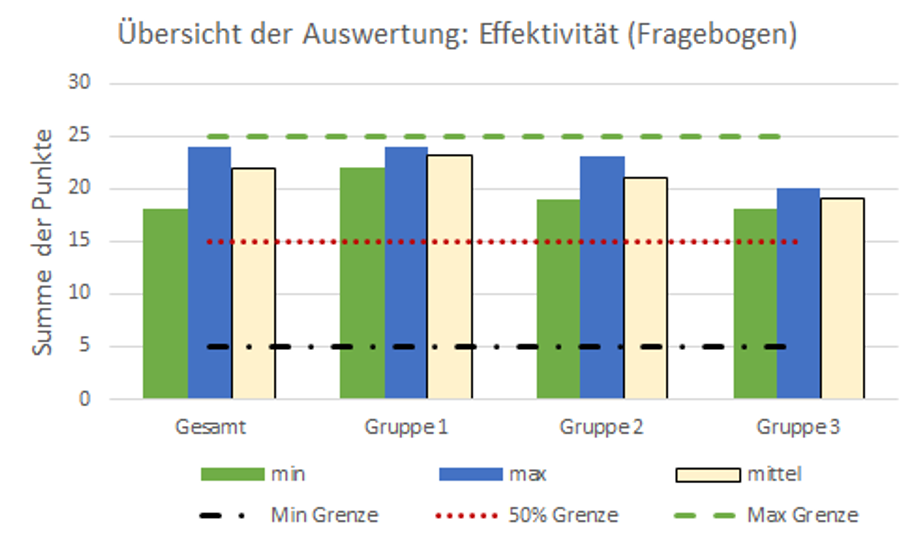
\includegraphics[width=0.9\linewidth]{img/Evaluation/Usability/AuswertungEffektivitaet}
\caption[Übersicht der Effektivität]{
	Auswertung Effektivität: Zeigt jeweils, nach Gruppen sortiert (siehe: \nameref{Stichproben}) und Gesamt (alle Gruppen), die summierten Punkte (Min. Punkte, Max. Punkte und Mittelwert Punkte) der Antworten aus dem Fragebogen, welche sich auf die Kategorie Effektivität beziehen. Quelle: eigene Ausarbeitung.
	}
\label{fig:AuswertungEffektivitaet}
\end{figure}


\subsubsection{Effizienz}
Zu der Kategorie Effizienz wurden im Fragebogen fünf Fragen gestellt, woraus sich ebenfalls folgende Grenzen definieren: Min. Grenze = 5 Punkte, Max. Grenze = 25 Punkte und 50\% Grenze = 15 Punkte\\
\\
Anhand dieser Grenzen und den Werten aus R\low{Effizienz} wurde das Diagramm \nameref{fig:AuswertungEffizienz} (siehe Abb.: \ref{fig:AuswertungEffizienz}) erstellt\footnote{Details siehe Abschnitt: \nameref{AufbauDiagramm}}.\\
\\
Der niedrigste Wert von allen R\low{Effizienz} liegt bei 20 Punkten und der größte Wert bei 25 Punkten.
Im Mittel lag R\low{Effizienz} in der Gruppe 1 bei 22,84 Punkten (Min. 21 Punkte und Max. 25 Punkte), in der Gruppe 2 bei 22,67 Punkten (Min. 20 und Max. 25 ) und in der Gruppe 3 bei 22 Punkten (Min. 21 und Max. 23)\\
(siehe Abb.: \ref{fig:AuswertungEffizienz}).

\paragraph{Resultat Effizienz} Da Min. R\low{Effizienz} mit 20 Punkten über der 50\% Grenze mit 15 Punkten liegt, wird K\low{Effizienz} positiv gewertet.

\begin{figure}[H]
\centering
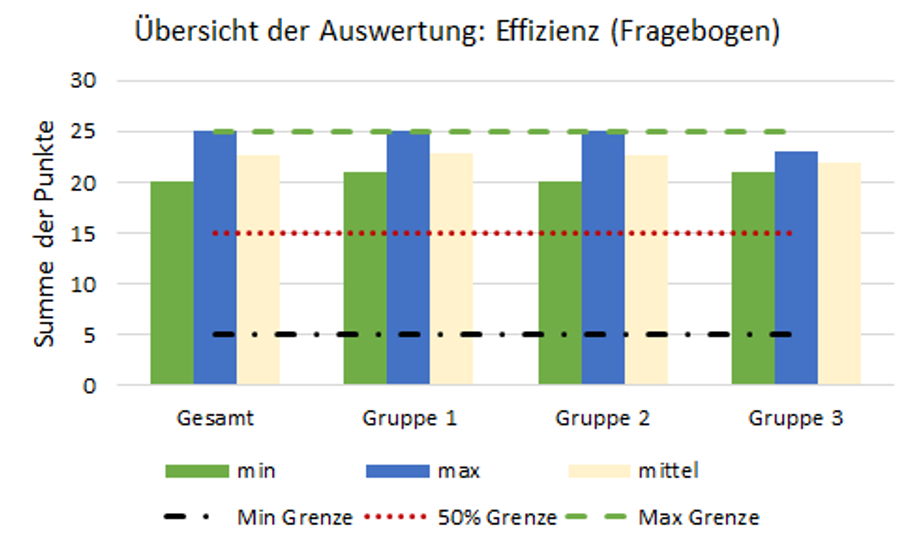
\includegraphics[width=0.9\linewidth]{img/Evaluation/Usability/AuswertungEffizienz}
\caption[Übersicht der Effizienz]{Auswertung Effizienz: Zeigt jeweils, nach Gruppen sortiert (siehe: \nameref{Stichproben}) und Gesamt (alle Gruppen), die summierten Punkte (Min. Punkte, Max. Punkte und Mittelwert Punkte) der Antworten aus dem Fragebogen, welche sich auf die Kategorie Effizienz beziehen. Quelle: eigene Ausarbeitung.}
\label{fig:AuswertungEffizienz}
\end{figure}


\subsubsection{Zufriedenheit}
Zu der Kategorie Zufriedenheit wurden im Fragebogen drei Fragen gestellt, woraus sich folgende Grenzen definieren: Min. Grenze = 3 Punkte, Max. Grenze = 15 Punkte und 50\% Grenze = 9 Punkte\\
\\
Anhand dieser Grenzen und den Werten aus R\low{Zufriedenheit} wurde das Diagramm \nameref{fig:AuswertungZufriedenheit} (siehe Abb.: \ref{fig:AuswertungZufriedenheit}) erstellt\footnote{Details siehe Abschnitt: \nameref{AufbauDiagramm}}.\\
\\
Der niedrigste Wert von allen R\low{Zufriedenheit} liegt bei 12 Punkten und der größte Wert bei 15 Punkten.
Im Mittel lag R\low{Zufriedenheit} in der Gruppe 1 bei 14,34 Punkten (Min. 13 Punkte und Max. 15 Punkte), in der Gruppe 2 bei 13,67 Punkten (Min. 12 und Max. 15 ) und in der Gruppe 3 bei 14,5 Punkten (Min. 14 und Max. 15)\\
(siehe Abb.: \ref{fig:AuswertungZufriedenheit}).

\paragraph{Resultat Zufriedenheit} Da Min. R\low{Zufriedenheit} mit 12 Punkten über der 50\% Grenze mit 9 Punkten liegt, wird K\low{Zufriedenheit} positiv gewertet.
\begin{figure}[H]
\centering
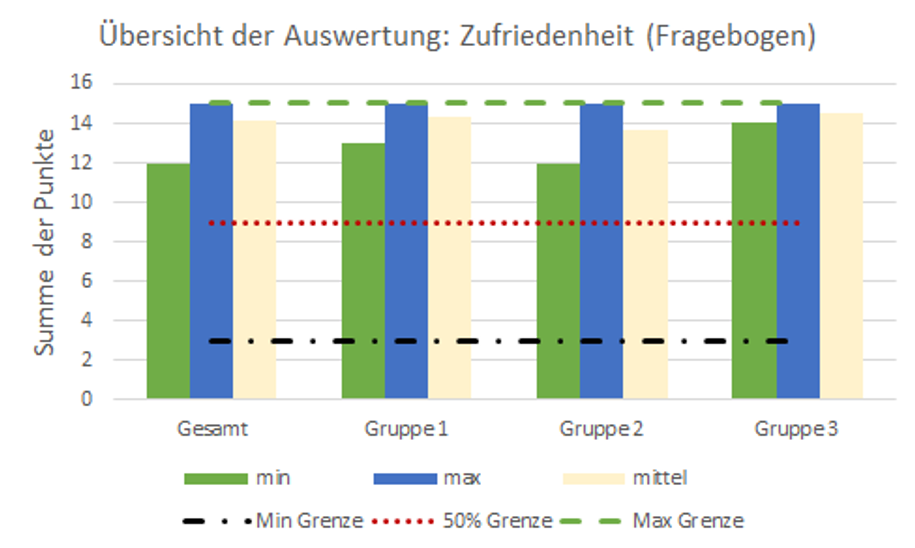
\includegraphics[width=0.9\linewidth]{img/Evaluation/Usability/AuswertungZufriedenheit}
\caption[Übersicht der Zufriedenheit]{Auswertung Zufriedenheit: Zeigt jeweils, nach Gruppen sortiert (siehe: \nameref{Stichproben}) und Gesamt (alle Gruppen), die summierten Punkte (Min. Punkte, Max. Punkte und Mittelwert Punkte) der Antworten aus dem Fragebogen, welche sich auf die Kategorie Zufriedenheit beziehen. Quelle: eigene Ausarbeitung.}
\label{fig:AuswertungZufriedenheit}
\end{figure}

\subsection{Eyetracking}
Aufgrund der dynamischen Webelemente (Karte zoomen und verschieben) konnte keine gruppenbasierte Analyse des Tests durchgeführt werden. 
Stattdessen wurden die Ergebnisse in erster Linie für die Analyse der \nameref{ergebnis_darstellungsformen} verwendet (siehe gleichnamigen Abschnitt). 

\subsection{Anmerkungen der Testpersonen}
\label{AnmerkungUser}
In diesem Abschnitt sollen die Anmerkungen der Testpersonen wiedergegeben und zusammengefasst werden. 
Während des Eyetracking-Tests wurden die Aussagen vom Testpersonal dokumentiert und im Anschluss an das Ausfüllen des Fragebogens noch einmal mit den Testpersonen besprochen.
Für einen besseren Überblick werden die jeweiligen Antworten, je nach Intention, in die Abschnitte positives Feedback und Optimierungspotential unterteilt. 

\paragraph{Positives Feedback}
10 von 11 Testpersonen haben sich während sowie nach dem Trip positiv zu der Unterstützung beim Planungsprozess geäußert. 
Davon haben zwei Testpersonen angegeben, dass der Prototyp alternativlos für das gegebene Testszenerio sei.  
Eine weitere Testperson gab an, dass das Maß an dargestellten Information optimal ausgewogen sei.

\paragraph{Optimierungspotential}
3 von 11 Testpersonen gaben an, dass sie in der Listenansicht Probleme hatten, ein Unternehmen zur Auswahl hinzuzufügen.
Dabei versuchten Sie das Unternehmen durch einen Klick auf den Namen, welcher als Link formatiert ist und zu Detailansicht des Kunden führt, zur Auswahl hinzuzufügen (siehe Abb.: \ref{fig:AddButton}).
Weitere fünf Testperson versuchten auf die gleiche Weise ein Unternehmen hinzuzufügen, äußerten aber sich nicht während des Testes dazu.

\begin{figure}[H]
	\centering
	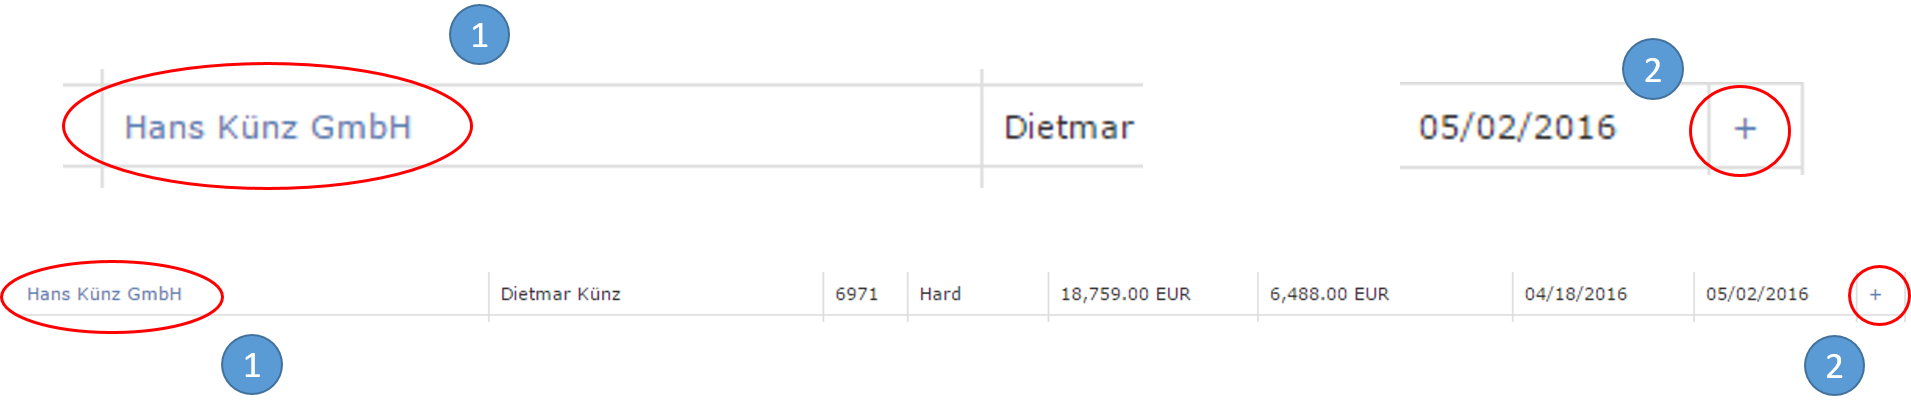
\includegraphics[width=1\linewidth]{img/Evaluation/Userfeedback/AddButton}
	\caption[Auschnitt Listenansicht]{Bildschirmfoto einer Zeile in der Listenansicht. Markierung 1: Name des Unternehmens als Link zur Detailansicht des entsprechenden Unternehmens. Markierung 2: Button mit der Beschriftung Plus (+) um das Unternehmen zur Auswahl hinzuzufügen. Sämtliche Zahlen sind fiktiv. Quelle: eigene Ausarbeitung.}
	\label{fig:AddButton}
\end{figure}
Da der Prototyp laut Definition mit englischer Benutzeroberfläche implementiert wurde, weicht das Datumsformat (englisch Monat/Tag/Jahr) dementsprechend vom deutschen Datumsformat (Tag.Monat.Jahr) ab. 
Für 3 von 11 Testperson war das englische Datumsformat so irritierend, dass es während des Tests angesprochen wurde.

\subsection{Verwendung und Einsatz der Darstellungsformen}
\label{ergebnis_darstellungsformen}
Für die Auswertungen der verwendeten Darstellungsformen dienen in erster Linie die Videomitschnitte des Eyetracking Tests. 
Dabei bearbeiteten die Testpersonen jeweils drei verschiedene Aufgabenstellungen, welche ein ansteigendes Komplexitätsniveau aufweisen.
Im folgenden Text werden die einzelnen Aufgabenstellungen als Trip bezeichnet.
\footnote{Eine Übersicht über die Aufgabenstellung des Eyetrackingtests findet sich im Abschnitt \ref{Verfahren} - \nameref{Verfahren}. Der vollständige Test befindet sich im Anhang (siehe Abschnitt \ref{anhangEyetracking} - \nameref{anhangEyetracking}). 
	}\\
	\\
Im ersten Schritt wurde, mit Hilfe des Videomitschnitts des Eyetrackings, die jeweilige Bearbeitungsdauer der einzelnen Trips pro Testperson ausgewertet und nach den entsprechenden Testgruppen gruppiert (siehe Abb.: \ref{fig:BearbeitungsdauerTrip}).  
Anhand dieser Datensätze wurde ausgewertet wie viel Zeit die einzelnen Testgruppen für die jeweiligen Trips benötigt haben.
Im Mittelwert lag die Bearbeitungsdauer für Trip 1 zwischen 54 Sekunden und 02:35 Minuten, für Trip 2 zwischen 01:20 Minuten und 03:09 Minuten sowie für Trip 3 zwischen 03:06 Minuten und 04:39 Minuten (siehe Abb.: \ref{fig:BearbeitungsdauerTrip}).
\begin{figure}[H]
\centering
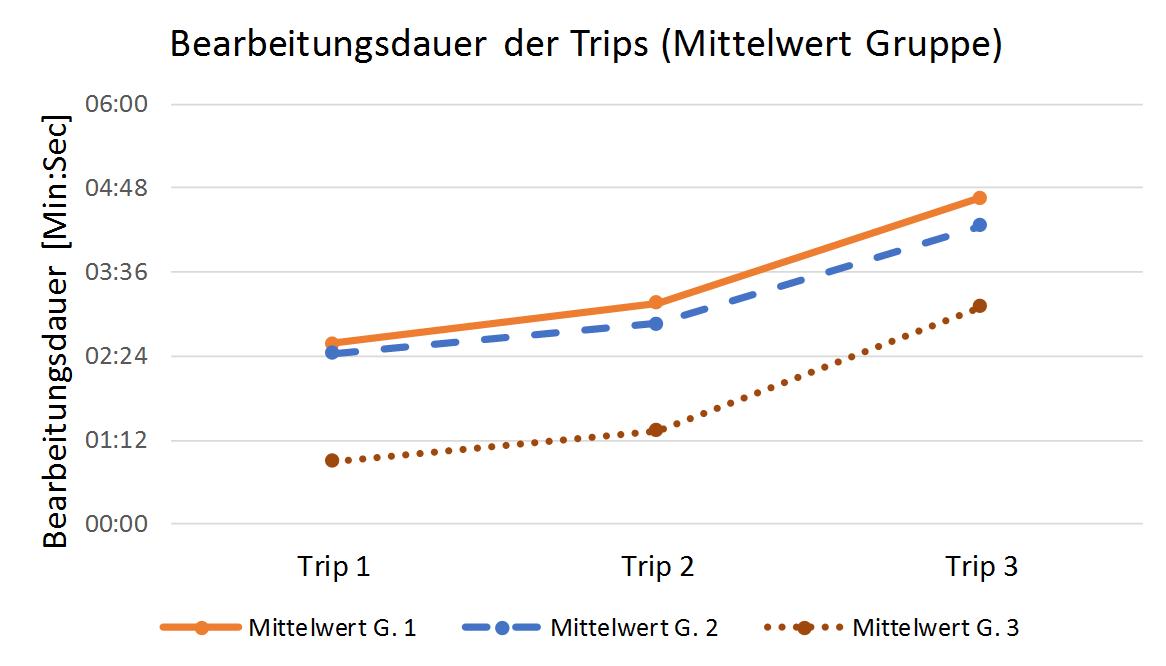
\includegraphics[width=0.7\linewidth]{img/Evaluation/Darstellungsformen/BearbeitungsdauerTrip}
\caption[Übersicht der Bearbeitungsdauer]{Übersicht der Bearbeitungsdauer der einzelnen Trips in Minuten. Die Daten entsprechen dem Mittelwert der jeweiligen Gruppen.  
Quelle: eigene Ausarbeitung.
	}
\label{fig:BearbeitungsdauerTrip}
\end{figure}

Um die Art und Weise, wie die Testpersonen die jeweiligen Darstellungsformen bei der Planung der Trips verwendet haben, besser zu verstehen, wurden im nächsten Schritt die Datensätze welche sich auf die Darstellungsarten beziehen untersucht. 
Dabei wurde analysiert wie viel Zeit alle Gruppen in Summe in den unterschiedlichen Ansichten verbracht haben (siehe Abb.: \ref{fig:VerwendungsdauerTrip}).
Um einen genaueren Einblick in die Verwendungsdauer zu erhalten wurden daraufhin die Daten zusätzlich nach den Testgruppen aufgeschlüsselt (siehe Abb.: \ref{fig:VerwendungsdauerGruppe}).
Ergänzend zum Aspekt der Zeit wurden die Anzahl der Wechsel zwischen den beiden Ansichten ausgewertet. 
Das Diagramm beschreibt wie oft (Mittelwert der Gruppe) innerhalb einer Gruppe eine Testperson die jeweilige Ansicht in den unterschiedlichen Trips aufgerufen hat (siehe Abb.: \ref{fig:Haufigkeit}). 

\begin{figure}[H]
\centering
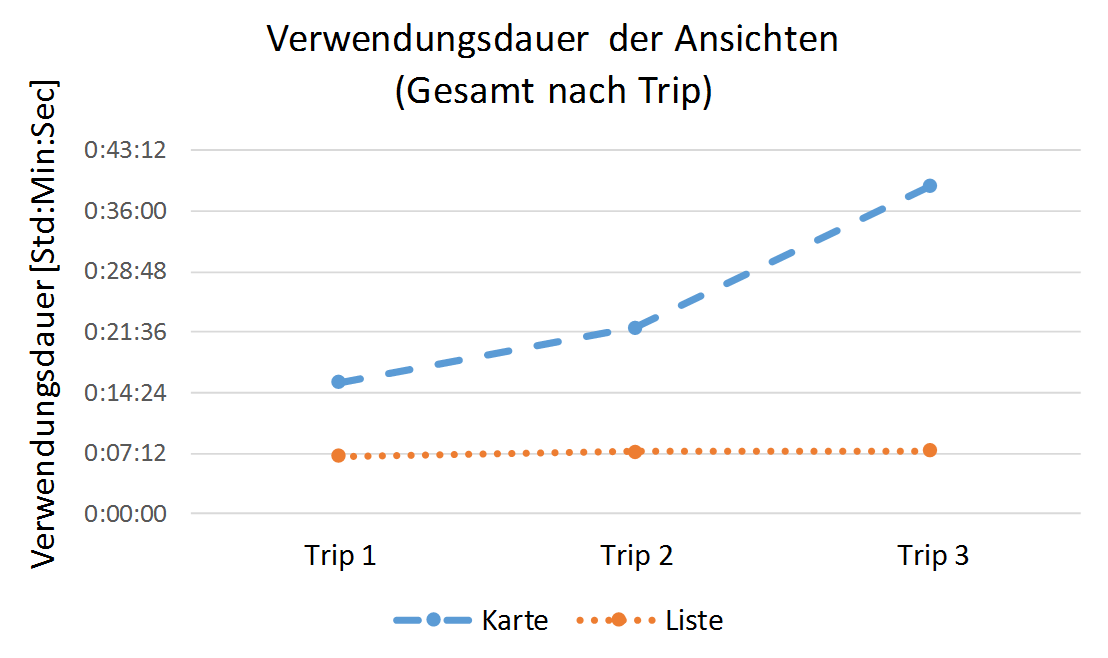
\includegraphics[width=0.7\linewidth]{img/Evaluation/Darstellungsformen/VerwendungsdauerTrip}
\caption[Verwendungsdauer der verschiedenen Ansichten.]{Übersicht über die Verwendungsdauer der verschiedenen Ansichten. Die Daten beziehen sich auf alle Gruppen (Summe) und wurden nach Trip gruppiert. Quelle: eigene Ausarbeitung.}
\label{fig:VerwendungsdauerTrip}
\end{figure}

\begin{figure}[H]
\centering
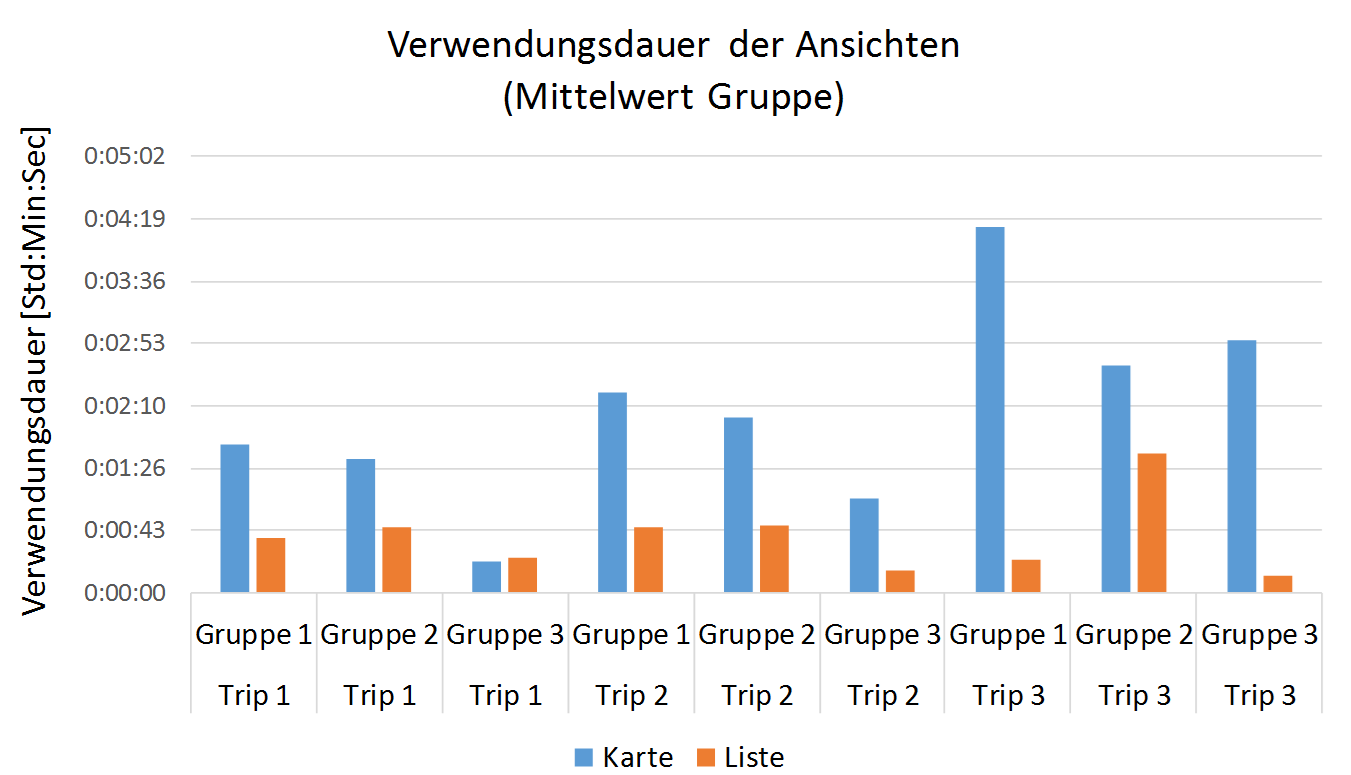
\includegraphics[width=0.7\linewidth]{img/Evaluation/Darstellungsformen/VerwendungsdauerGruppe}
\caption[Übersicht Verwendungsdauer Ansichten (Detail)]{Verwendungsdauer der verschiedenen Ansichten im Detail. Es wurden die Daten sowohl nach Gruppe (Mittelwert der Gruppe) als auch nach Trip gruppiert. Quelle: eigene Ausarbeitung.}
\label{fig:VerwendungsdauerGruppe}
\end{figure}

\begin{figure}[H]
\centering
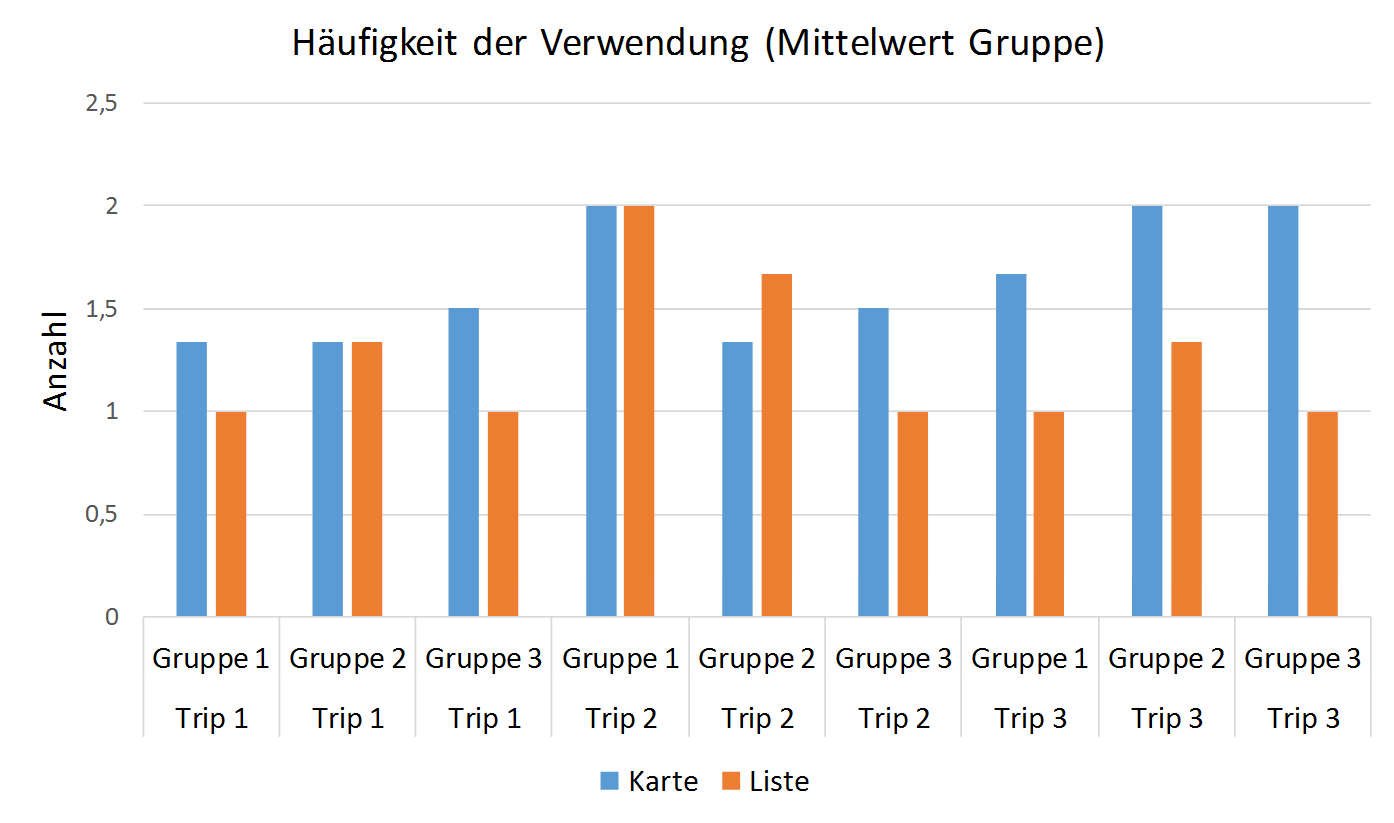
\includegraphics[width=0.7\linewidth]{img/Evaluation/Darstellungsformen/Haufigkeit}
\caption[Häufigkeit der der verwendeten Ansichten]{Übersicht über die Häufigkeit der Aufrufe der verschiedenen Ansichten. Das Diagramm zeigt an wie oft (Mittelwert) die jeweilige Ansicht in dem entsprechenden Trip aufgerufen wurde. Die Daten sind nach der Gruppe sowie nach Trip gruppiert. Quelle: eigene Ausarbeitung.}
\label{fig:Haufigkeit}
\end{figure}
\newpage
\subsubsection{Meilensteine}
\label{Meilensteine} 
Für den letzten Schritt der Auswertung wurden für jeden Trip eigene Meilensteine definiert. 
Die einzelnen Meilensteine kennzeichnen einen Teilerfolg innerhalb der Planung eines Trips (erste Ziffer: zugehöriger Trip, zweite Ziffer: aufsteigende Nummerierung) und wurden wie folgt definiert:

\begin{itemize}
	\item Trip 1
	\item[] M1-1: Auswahl des genannten Kontaktes 
	\item Trip 2
	\item[] M2-1: Auswahl des genannten Kontaktes
	\item[] M2-2: Auswahl des gesuchten Kontaktes
	\item Trip 3
	\item[] M3-1: Auswahl des genannten Kontaktes
	\item[] M3-2: Auswahl des ersten gesuchten Kontaktes
	\item[] M3-3: Auswahl des zweiten gesuchten Kontaktes
	\item[] M3-4: Auswahl des dritten gesuchten Kontaktes
\end{itemize}
Anhand des Videomaterials des Eyetrackings wurde untersucht, welche Ansicht beim Erreichen der jeweiligen Meilensteine von den Testpersonen verwendet wurde. 
Um die Ergebnisse dieser Auswertung zu visualisieren wurde das Diagramm \ref{fig:Meilenstein} angefertigt. 
Für diesen Zweck wurden die ausgewerteten Daten nach Gruppe (Mittelwert) und Meilenstein gruppiert.
Dabei ist zu beachten, das die Daten in der Y-Achse gestapelt abgebildet wurden und der Wert 1 auf der Y-Skala 100\% entspricht. 

\begin{figure}[h]
\centering
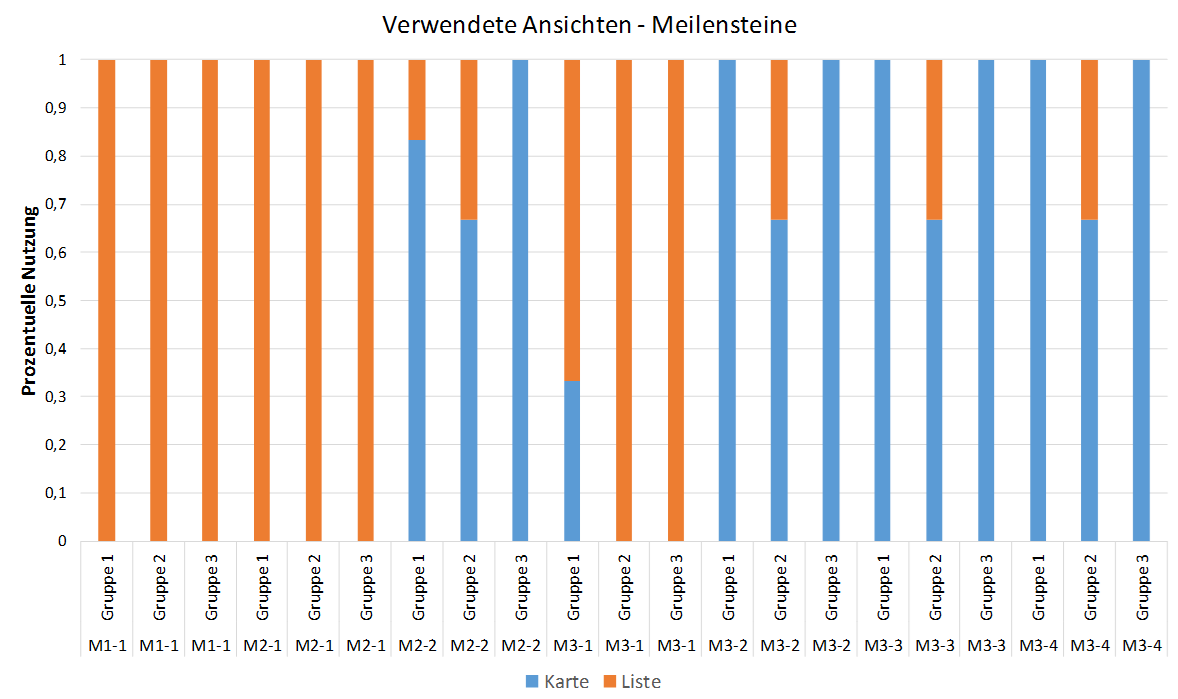
\includegraphics[width=1\linewidth]{img/Evaluation/Meilenstein}
\caption[Verwendete Ansichten - Meilensteine]{
	Übersicht über die verwendeten Ansichten beim erreichen des jeweiligen Meilensteins. Die Daten sind Mittelwerte über die jeweiligen Testgruppen und nach Meilensteinen sortiert (siehe Abschnitt \nameref{Meilensteine} für weitere Details). Y-Achse: die Daten werden gestapelt dargestellt, der Wert 1 entspricht 100\%.
	Quelle: eigene Ausarbeitung
	}
\label{fig:Meilenstein}
\end{figure}



\section{Interpretation \& Diskussion}
\label{InterpretationDiskussion}
Nachdem im letzten Abschnitt die Ergebnisse des Tests präsentiert wurden, sollen an dieser Stelle mögliche Interpretationen dieser Informationen besprochen werden.

\subsection{Usability Analyse}
Wie in dem entsprechenden Abschnitt bereits dargelegt wurde, erreichten alle drei Kategorien einen positives Ergebnis. 
Daraus kann geschlossen werden das die Usability (im Rahmen der Definition Gebrauchstauglichkeit) gegeben ist. 
Anhand der Testergebnisse, in denen alle drei Kategorien als positiv definiert wurden kann die Hypothese als bestätigt angesehen werden.  
\\
\\
Bei der Auswertung der Fragebögen ist aufgefallen, dass bei zwei Fragen der Mittelwert der Antworten unter 4 von 5 Punkten liegt. 
Dies ist zum einen der Irritation der Testpersonen beim Hinzufügen von Unternehmen zur Auswahl in der Listenansicht (Mittelwert 3,9 von 5 Punkten) und zum anderen dem ungewohnten englischen Datumsformat (Mittelwert 3,82 von 5 Punkten) geschuldet.
Diese beiden Punkte werden im nächstem Abschnitt näher behandelt.

\subsection{Anmerkungen der Testpersonen}
Bei der Analyse sind die drei Themen Hinzufügen von Unternehmen in der Listenansicht, englisches Datumsformat und der Wunsch nach einer Filterfunktion am deutlichsten hervorgetreten.\\
\newpage
\subsubsection*{Hinzufügen in der Listenansicht}
Innerhalb der Listenansicht, trat immer wieder bei verschiedenen Testpersonen Verwirrung auf, als sie sich unerwartet in der Detailansicht des Unternehmens wiederfanden und nicht wie vermutet das entsprechende Unternehmen zur Auswahl hinzugefügt wurde.
\\
\\
Diese Erwartungshaltung ist womöglich dem Umstand geschuldet, dass die betroffenen Testpersonen in ihrem geistigen Modell die Funktion des Hinzufügens mit dem exponiert stehenden (links in der Zeile), als Link formatierten, Unternehmensnamen assoziieren. \\
\\
Um dies besser zu verstehen muss der Aufbau der Listenansicht, im Speziellen die Anordnung der Elemente in einer Zeile
\footnote
{
	Anmerkung: Jede Zeile bildet in der Listenansicht ein Unternehmen ab.
}
, betrachtet werden.
Bei der Erstellung des Konzeptes wurde entschieden, nur die notwendigen Informationen abzubilden. Aus dieser Motivation heraus wurde der Name des Unternehmens in beiden Ansichten als Link gestaltet (siehe Abbildung: \ref{fig:AddButton}-1), welcher die Detailansicht aufruft, falls weitere Informationen zum entsprechenden Unternehmen gewünscht werden.
\\
\\
Des Weiteren wurde aus Gründen der Konsistenz (vgl. \cite[S. 103, 11:4 Ensure Visual Consistency]{Koyani2004}), in der Listenansicht der eigentliche Button zum Hinzufügen im rechten Bereich der Zeile, innerhalb der Listenansicht, platziert (siehe Abbildung \ref{fig:AddButton}-2)\footnote{
	Innerhalb von Pery sind Funktionen welche sich auf Zeilen in Listen beziehen (bearbeiten, löschen, etc.) rechts platziert.
	} 
und mit einem Plus (+) beschriftet, wie auch im Popup der Kartenansicht (siehe Abbildung: \ref{fig:Add}).
\newpage
Folgende Begründungen könnten die Ursache dafür sein, dass die Testpersonen den Link des Unternehmensnamens verwendet haben und nicht den bereitgestellten Button:

\begin{itemize}
	\item \textbf{Positionierung} Der Hinzufügen Button ist zwar nicht außerhalb des Sichtfeldes gelegen, allerdings ist der Unternehmensname, mit der Positionierung als zweites Element von links, deutlich hervorstechender. Eine Beobachtung dabei ist, dass sich selbst versierte Pery-Nutzer\_innen beim ersten Mal ähnlich verhalten haben.
	\item \textbf{Geistiges Modell} Testpersonen sind durch das erlernte Verhalten im Umgang mit Webseiten daran gewöhnt, dass ein Link (Unternehmensname) eine Funktion, im Normalfall eine Weiterleitung, ausführt.
	\item \textbf{Ausprägung} Die Gespräche mit den betroffenen Personen ergaben, dass der Button nicht als markant genug wahrgenommen wurde.
	\item \textbf{Unklarheit der Funktion} Testpersonen waren sich nicht im Klaren darüber welche Funktion der Button in der Listenansicht auslöst. Allerdings war allen Testpersonen der Verwendungszweck des Buttons innerhalb Kartenansicht sofort verständlich.
\end{itemize}
Mögliche Optimierungsvorschläge können unter anderem eine Änderung der Position und/oder die Änderung der Beschriftung in Hinzufügen, wodurch zum einen mehr Aufmerksamkeit auf den Button gelenkt wird und zum anderen die Bedeutung klarer wird. Die Bedeutung des Buttons in der Kartenansicht war allen Testpersonen klar, dementsprechend kann die Erscheinung des Buttons in der Listenansicht durch die Farbgebung an die Erscheinung in der Kartenansicht angepasst werden, um so Wiedererkennungswert zu schaffen.

\begin{figure}[h]
	\centering
	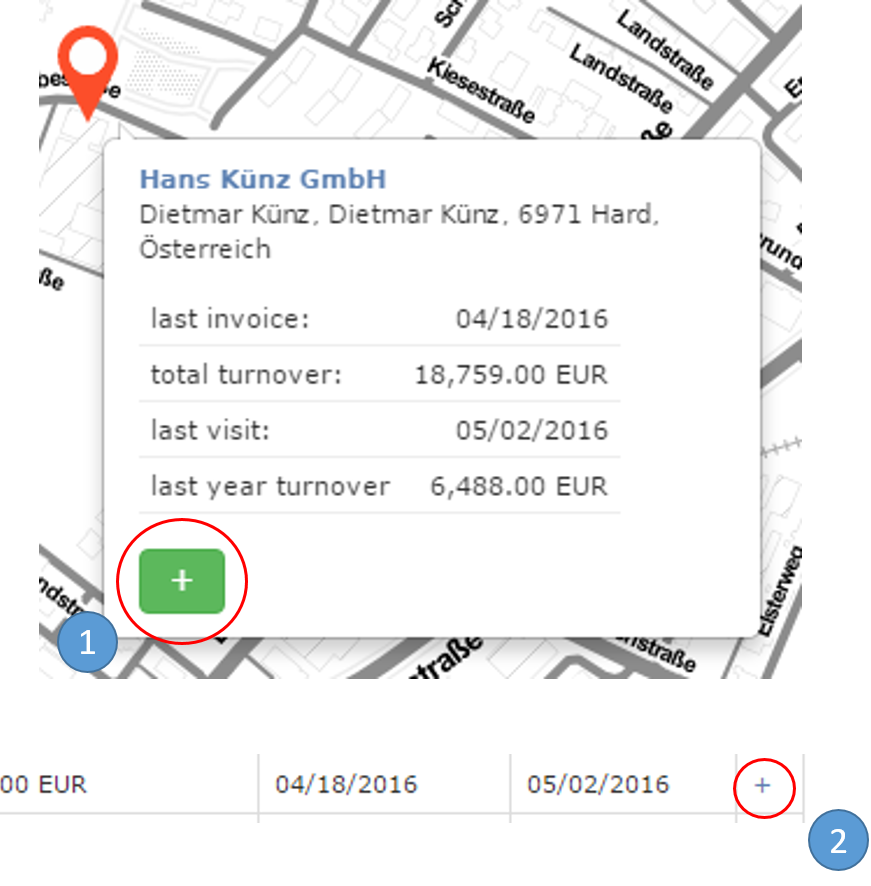
\includegraphics[width=0.7\linewidth]{img/Evaluation/Userfeedback/Add}
	\caption[Vergleich: Button Karte- und Listenansicht]{Vergleich: Hinzufügen von Unternehmen (Button). Markierung 1: Button im Popup der Kartenansicht, Markierung 2: Button in der Listenansicht. Die angegebenen Daten auf der Abbildung sind fiktiv. Quelle: eigene Ausarbeitung.}
	\label{fig:Add}
\end{figure}

\subsubsection*{Datumsformat}
Da die gesamte Benutzeroberfläche in Englisch gehalten ist wurde dementsprechend auch das englische Datumsformat (Monat/Tag/Jahr in Ziffern) verwendet. 
Das hat einen Teil der Testpersonen in einem solchen Ausmaß irritiert, dass die Kategorie Effizienz merkbar gelitten hat, da sie jedes mal geistig das gegebene Datum in das verwendete Datumsformat des Prototypen übertragen mussten und umgekehrt.\\
\\
Als möglicher Optimierungsansatz könnten die Ziffern des Monatsformates durch eine Abkürzung des Monatsnamens ersetzt werden wie Beispielsweise: Oct. 10, 2016 wodurch ein Verwechseln der Monats- und Tagesziffer ausgeschlossen wird.  
\\
\\
An dieser Stelle ist anzumerken, dass alle Testpersonen Deutsch als Muttersprache sprechen.

\subsubsection*{Filterfunktion}
Drei von elf Personen an, dass sie sich eine Filterfunktion wünschen, um einen besseren Überblick bei der Planung zu erhalten gaben .  
Diese Filterfunktion wurde sowohl für die Karten- als auch für die Listenansicht gewünscht.
Innerhalb der Kartenansicht sollen dabei Marker und in der Listenansicht dementsprechend Zeilen ausgeblendet werden.
 

\subsection{Verwendung und Einsatz der Darstellungsformen}
Die Kombination der unterschiedlichen Datenvisualisierungen (Karten- und Listenansicht) in Verbindung mit der Anreicherung der Kerndaten mit kontextsensitiven Daten ist von den Testpersonen sehr gut angenommen und im Fragebogen bekundet worden (siehe Abschnitt: \nameref{Ergebnisse}).
Der nachfolgende Abschnitt beschäftigt sich speziell damit, ob die gemessen Werte des Eyetracking Tests zu übereinstimmenden bzw. ähnlichen Ergebnissen kommen,  wie die subjektive Bewertung der Testpersonen.
\pagebreak
Als erster Schritt soll im Vorfeld die Bearbeitungsdauer der einzelnen Trips betrachtet werden, da sie als Grundlage für die weiteren Annahmen dient. 
Dabei ist zu erkennen, dass die mittlere Bearbeitungsdauer bei allen Testpersonen nach einem ähnlichen Muster ansteigt (siehe Abb. \ref{fig:BearbeitungsdauerTrip}).
Außerdem fällt dabei auf, dass sich die Erfahrung im Umgang mit Pery auf die Bearbeitungsdauer niederschlägt. 
Die Gruppe mit der meisten Erfahrung in Pery (Gruppe 3) erledigte die Aufgaben am schnellsten, gefolgt von der Gruppe mit mittleren Erfahrungsgrad (Gruppe 2), während die Gruppe ohne Erfahrungen (Gruppe 3) im Umgang mit Pery am Längsten brauchte (siehe Abb. \ref{fig:BearbeitungsdauerTrip}).
Dabei ist zu betonen, dass es sich hierbei um eine Auffälligkeit handelt und für eine Bestätigung weitere Tests durchgeführt werden müssten.\\
\\
Bei der Auswertung der absoluten Verwendungsdauer ist zu erkennen (siehe Abb. \ref{fig:VerwendungsdauerTrip}), dass die Verwendungsdauer (Mittelwert aller Testpersonen) der Kartenansicht\footnote{Verwendungsdauer der Kartenansicht Trip 1: ca. 15 min., Trip 2: ca. 22 min. und Trip 3: ca. 39 min.} im Gegensatz zur Listenansicht\footnote{Verwendungsdauer der Listenansicht: zwischen 6:48 min. und 7:31 min.} stetig ansteigt.  
Im Detail werden die gleichen Daten nach Testgruppen gruppiert in Abbildung \ref{fig:VerwendungsdauerGruppe} dargestellt. 
Darauf ist zu erkennen, dass die Testgruppen - bis auf eine Ausnahme - mehr Zeit in der Kartenansicht als in der Listenansicht zum Lösen der Aufgabenstellungen verbracht haben. 
Diese Ausnahme stellt die Gruppe 2 in Trip 1 dar: Dies ist die einzige Situation, in der der Mittelwert der Verwendungszeit einer Gruppe in der Listenansicht höher ist als in der Kartenansicht (Kartenansicht: 22 Sec. und Listenansicht 23 Sec.).
\\
\\
Mit dem Ansteigen der Komplexität (siehe Abb. \ref{fig:VerwendungsdauerTrip}), steigt gleichzeitig die Nutzungsdauer der Kartenansicht in einem ähnlichen Muster (siehe Abb. \ref{fig:VerwendungsdauerGruppe}).
\\
\\
Ergänzend zu der Dauer soll die Anzahl der Wechsel zwischen den einzelne Ansichten betrachtet werden (siehe Abb. \ref{fig:Haufigkeit}).
Alle Gruppen haben sowohl die Karten- als auch die Listenansicht zum Lösen der Aufgabenstellungen verwendet. 
In Trip 3 wurde allerdings am häufigsten zu der Kartenansicht gewechselt. \\
\\
Zusätzlich zu den einzelnen Trips wurden Meilensteine definiert welche Teilerfolge innerhalb der Trips darstellen.
\footnote{
	Die Definition der einzelnen Meilensteine können im gleichnamigen Abschnitt der Sektion \nameref{Ergebnisse} nachgeschlagen werden.
	}
Anhand der Auswertungen ist ersichtlich, welcher Meilenstein mit welcher Ansicht erreicht wurde (siehe Abb. \ref{fig:Meilenstein}). 
Dabei ist zu beachten, dass hierbei nur die Ansicht genannt wird, welche zum Zeitpunkt des Erreichens aktiv war und nicht welche Ansichten wie lange davor verwendet wurden, um diesen Meilenstein zu erreichen.
Dabei ist zu beobachten, dass bei allen Meilensteinen, in denen nur ein Wert gesucht wurde (Unternehmensname oder Gesamtumsatz), bei allen Gruppen der Einsatz der Listenansicht überwiegt. (siehe Abb. \ref{fig:Meilenstein} - Meilenstein: M1-1, M2-1 und M3-1).
Dementsprechend steigt der Anteil Kartenansicht zum Lösen der komplexeren Meilensteine deutlich an (siehe Abb. \ref{fig:Meilenstein} - Meilenstein:  M2-2 und M3-2 bis M3-4).  \\
\\
Abschließend lässt sich zu der Auswertung der unterschiedlichen Darstellungsformen folgende Erkenntnisse zusammenfassen: 
\begin{itemize}
	\item[] Die Verwendung der jeweiligen Ansicht ist an die Komplexität bzw. die Art der  Aufgabenstellung gebunden.
	\item[] Bei Aufgabenstellungen mit einer einzelnen Bedingung (siehe Trip 1 sowie erster Teil von Trip 2 und Trip 3) wurde bevorzugt die Listenansicht gewählt.
	\item[] Bei Aufgabenstellungen mit mehreren Bedingungen und/oder geografischen Abhängigkeiten (siehe zweiter Teil von Trip 2 und Trip 3) wurde bevorzugt die Kartenansicht eingesetzt. 
\end{itemize}

Schlussendlich ergänzt die Kartenansicht somit zwar die konservative Listenansicht sinnvoll, ersetzt diese aber in der Form dieses Prototypen nicht. Die Kartenansicht wurde besonders zum Lösen komplexerer Aufgaben genutzt. Die Kartenansicht bietet einerseits eine bessere geografische Orientierung über die Standorte, andererseits auch eine grobe Übersicht über die Ranks der Unternehmen.

\end{document}